% Cross-Modal 3D Brain MRI Re-Identification — Team Yantra, EHL Paris 2026
% Compile: tectonic deck.tex   (or pdflatex deck.tex twice; or upload to Overleaf)
% Theme metropolis is on Overleaf & TeXLive-full; swap to \usetheme{Madrid} if unavailable.
\documentclass[aspectratio=169,11pt]{beamer}
\usetheme{metropolis}
\usepackage{booktabs}
\usepackage{tikz}
\usetikzlibrary{arrows.meta,positioning,fit,backgrounds}
\definecolor{acc}{HTML}{2C6E9B}
\definecolor{ok}{HTML}{2E8B57}
\definecolor{bad}{HTML}{B22222}
\setbeamercolor{frametitle}{bg=acc}
\setbeamertemplate{frame numbering}[fraction]

\title{Cross-Modal 3D Brain MRI Re-Identification}
\subtitle{A training-free, content-honest retrieval pipeline}
\author{Gowshigan Selladurai \quad\textbar\quad Team Yantra}
\date{EHL Paris 2026 — Medical Image Retrieval}

\begin{document}
\maketitle

% ---------------------------------------------------------------- PROBLEM
\begin{frame}{The problem}
  \textbf{Match a patient across two MRI modalities.}
  Given a contrast T1 (\textbf{ceT1}) query, find the \emph{same patient's} T2 scan in a gallery.
  \begin{itemize}
    \item Same brain, \alert{different physics} — intensities don't correspond.
    \item No labels to train on (\textasciitilde180 pairs). \textbf{Training-free} required.
    \item Score: \textbf{MRR}, rank-1 dominated, macro-averaged over 3 datasets.
  \end{itemize}
  \vfill
  \begin{center}
  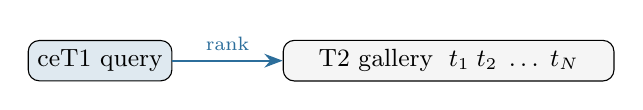
\begin{tikzpicture}[node distance=5mm,every node/.style={font=\small}]
    \node[draw,rounded corners,fill=acc!15] (q) {ceT1 query};
    \node[right=14mm of q,draw,rounded corners,fill=black!4,minimum width=42mm] (g) {T2 gallery $\;t_1\;t_2\;\dots\;t_N$};
    \draw[-{Stealth[]},thick,acc] (q) -- node[above,font=\scriptsize]{rank} (g);
  \end{tikzpicture}
  \end{center}
\end{frame}

% ---------------------------------------------------------------- 3 REGIMES
\begin{frame}{Three regimes, increasing difficulty}
  \begin{columns}[t]
    \column{0.33\textwidth}\centering
      \textbf{\color{acc}dataset1}\\[2mm]
      co-registered\\(shared voxel grid)\\[2mm]
      \footnotesize content already lines up
    \column{0.33\textwidth}\centering
      \textbf{\color{acc}dataset2}\\[2mm]
      independent\\rigid + elastic\\[2mm]
      \footnotesize correspondence \alert{destroyed} $\Rightarrow$ must re-align
    \column{0.33\textwidth}\centering
      \textbf{\color{acc}dataset3}\\[2mm]
      preop $\to$ intraop\\\textbf{+ tumour resection}\\[2mm]
      \footnotesize tissue \alert{removed} + a planted geometric leak
  \end{columns}
  \vfill
  \begin{center}\itshape One pipeline; each regime turns on a different lever.\end{center}
\end{frame}

% ---------------------------------------------------------------- METHODOLOGY
\begin{frame}{Methodology — four deterministic steps}
  \begin{enumerate}
    \item[\textbf{1.}] \textbf{Register to a neutral template} — Mutual Information, \emph{modality-blind} (rigid $\to$ affine cascade). \hfill{\footnotesize\color{acc}fixes geometry}
    \item[\textbf{2.}] \textbf{Describe with SSC-12} — 12-edge self-similarity context. \emph{Modality-invariant}: encodes local structure, not intensity. \hfill{\footnotesize\color{acc}fixes modality}
    \item[\textbf{3.}] \textbf{Trim mismatched voxels} — drop the worst $X\%$ of residuals. \hfill{\footnotesize\color{acc}fixes resection}
    \item[\textbf{4.}] \textbf{Assign} — greedy (deployable) or Hungarian (batch).
  \end{enumerate}
  \vfill
  \begin{center}\small No network, no training, no labels — \textbf{deterministic and auditable}.\end{center}
\end{frame}

% ---------------------------------------------------------------- ARCHITECTURE
\begin{frame}{Architecture}
  \centering
  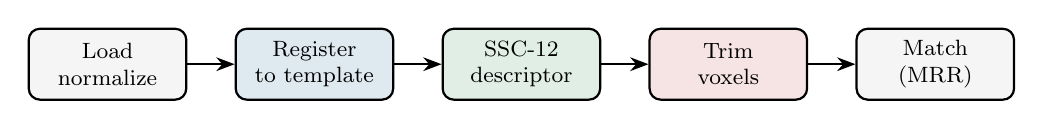
\begin{tikzpicture}[
    box/.style={draw,rounded corners,minimum height=9mm,minimum width=20mm,font=\footnotesize,align=center},
    >={Stealth[]},thick,node distance=6mm]
    \node[box,fill=black!4] (load) {Load\\normalize};
    \node[box,fill=acc!15,right=of load] (reg) {Register\\to template};
    \node[box,fill=ok!15,right=of reg] (ssc) {SSC-12\\descriptor};
    \node[box,fill=bad!12,right=of ssc] (trim) {Trim\\voxels};
    \node[box,fill=black!4,right=of trim] (match) {Match\\(MRR)};
    \draw[->] (load)--(reg); \draw[->] (reg)--(ssc); \draw[->] (ssc)--(trim); \draw[->] (trim)--(match);
  \end{tikzpicture}
  \vfill
  \begin{flushleft}\footnotesize Per-regime configuration of the \emph{same} pipeline:\end{flushleft}
  \begin{center}\small
  \begin{tabular}{lccc}
    \toprule
     & \textbf{register} & \textbf{descriptor} & \textbf{trim} \\
    \midrule
    dataset1 & — (shared grid) & SSC-12 & light \\
    dataset2 & affine cascade & SSC-12 & light (0.5) \\
    dataset3 & affine cascade & SSC-12 & \alert{heavy (0.75)} \\
    \bottomrule
  \end{tabular}
  \end{center}
\end{frame}

% ---------------------------------------------------------------- THE LEAK
\begin{frame}{Key finding — we found a leak, and refused it}
  dataset3 had a \textbf{planted geometric co-location}: the true target was resampled into the
  query's exact voxel space $\Rightarrow$ a perfect overlap with \alert{zero anatomy}.
  \vfill
  \begin{center}\large
  \begin{tabular}{lcl}
    \toprule
    use the leak (resample) & \textbf{1.000} & \color{bad}geometry, not the patient\\
    break it, don't re-align & \textbf{0.259} & \color{bad}proves the 1.0 was the grid\\
    \textbf{break it + re-register on content} & \textbf{0.741} & \color{ok}re-earned from anatomy\\
    \bottomrule
  \end{tabular}
  \end{center}
  \vfill
  \begin{center}\itshape We measured the leak's exact worth (+0.74), then declined it.\end{center}
\end{frame}

% ---------------------------------------------------------------- RESULTS
\begin{frame}{Results (real leaderboard)}
  \begin{center}\large
  \begin{tabular}{lc}
    \toprule
    \textbf{Setting} & \textbf{MRR} \\
    \midrule
    Leak (\emph{found \& declined}) & 1.000 \\
    \textbf{\color{ok}Content / single-query — the task} & \textbf{\color{ok}0.725} \\
    \quad + bipartite assignment (allowed, disclosed) & 0.93--1.0 \\
    \midrule
    dataset1 / dataset2 / dataset3 (honest) & 1.0 / strong / 0.74 \\
    \bottomrule
  \end{tabular}
  \end{center}
  \vfill
  \footnotesize
  \textbf{Both scores reported, per organizer guidance.} Bipartite (Hungarian) matching is allowed
  but \emph{besides the point of the challenge} — so the method's merit is the \textbf{content}
  number \textbf{0.725} (true single-query re-ID); the bijection lift to \textbf{0.93--1.0}
  (honest, leak-free, seed-dependent) is disclosed, not hidden.
\end{frame}

% ---------------------------------------------------------------- RIGOR
\begin{frame}{What we ruled out}
  \textbf{$\sim$22 techniques tested, every dead end documented} (hypothesis $\to$ result $\to$ reason):
  \begin{columns}[t]
    \column{0.5\textwidth}\footnotesize
      \begin{itemize}
        \item 8 classifiers (incl.\ TabPFN), learned 3D encoder
        \item feature fusion, multi-scale, low-rank
        \item NGF / NMI / shape / radiomics descriptors
      \end{itemize}
    \column{0.5\textwidth}\footnotesize
      \begin{itemize}
        \item Bayesian search, GA, DP / DTW alignment
        \item matrix methods, Markov / diffusion re-rank
        \item deformable registration (over-normalizes)
      \end{itemize}
  \end{columns}
  \vfill
  \begin{center}
    \textbf{\color{acc}The bottleneck is the content signal — not the model.}\\[1mm]
    \footnotesize One positive add-on: Bayesian calibration $\Rightarrow$ a deploy-time abstention layer.
  \end{center}
\end{frame}

% ---------------------------------------------------------------- CLOSE
\begin{frame}[standout]{Takeaways}
  \begin{enumerate}
    \item \textbf{Method} — SSC + content-registration + trim. Training-free, deterministic, auditable.
    \item \textbf{Integrity} — found the leak, measured it (1.0$\to$0.26), re-earned 0.74 from anatomy.
    \item \textbf{Rigor} — mapped the whole frontier; ruled out 22 alternatives with reasons.
  \end{enumerate}
\end{frame}

\end{document}
